%%
%% This is file `main.tex' based on `sample-sigconf.tex' (q.v. for spurce of that,
%%
%% IMPORTANT NOTICE:
%% 
%% For the copyright see the original source file `sample-sigconf.tex'
%% in the `Sample' folder.
%%
%% For distribution of the original source see the terms
%% for copying and modification in the file samples.dtx.
%% 
%% This generated file may be distributed as long as the
%% original source files, as listed above, are part of the
%% same distribution. (The sources need not necessarily be
%% in the same archive or directory.)
%%
%% Commands for TeXCount
%TC:macro \cite [option:text,text]
%TC:macro \citep [option:text,text]
%TC:macro \citet [option:text,text]
%TC:envir table 0 1
%TC:envir table* 0 1
%TC:envir tabular [ignore] word
%TC:envir displaymath 0 word
%TC:envir math 0 word
%TC:envir comment 0 0
%%
%%
%% The first command in your LaTeX source must be the \documentclass command.

%% NOTE that a single column version is required for 
%% submission and peer review. This can be done by changing
%% the \doucmentclass[...]{acmart} in this template to 
%%\documentclass[manuscript,review,anonymous]{acmart}
%% This version is used for drafting and final submission
\documentclass[sigconf]{acmart}


%% 
%% To ensure 100% compatibility, please check the white list of
%% approved LaTeX packages to be used with the Master Article Template at
%% https://www.acm.org/publications/taps/whitelist-of-latex-packages 
%% before creating your document. The white list page provides 
%% information on how to submit additional LaTeX packages for 
%% review and adoption.
%% Fonts used in the template cannot be substituted; margin 
%% adjustments are not allowed.

%%
%% Submission ID.
%% Use this when submitting an article to a sponsored event. You'll
%% receive a unique submission ID from the organizers
%% of the event, and this ID should be used as the parameter to this command.
%%\acmSubmissionID{123-A56-BU3}

%%
%% For managing citations, it is recommended to use bibliography
%% files in BibTeX format.
%%
%% You can then either use BibTeX with the ACM-Reference-Format style,
%% or BibLaTeX with the acmnumeric or acmauthoryear sytles, that include
%% support for advanced citation of software artefact from the
%% biblatex-software package, also separately available on CTAN.
%%
%% Look at the sample-*-biblatex.tex files for templates showcasing
%% the biblatex styles.
%%

%%
%% The majority of ACM publications use numbered citations and
%% references.  The command \citestyle{authoryear} switches to the
%% "author year" style.
%%
%% If you are preparing content for an event
%% sponsored by ACM SIGGRAPH, you must use the "author year" style of
%% citations and references.
%% Uncommenting
%% the next command will enable that style.
%%\citestyle{acmauthoryear}

%%
%% end of the preamble, start of the body of the document source.

%% % Location of your graphics files for figures, here a sub-folder to the main project folder
\graphicspath{{./images/}} 

\begin{document}

%%
%% The "title" command has an optional parameter,
%% allowing the author to define a "short title" to be used in page headers.
\title{Ghost in the Shell - Using Runtime Profiling and LLMs for Code Improvement}

%%
%% The "author" command and its associated commands are used to define
%% the authors and their affiliations.
%% Of note is the shared affiliation of the first two authors, and the
%% "authornote" and "authornotemark" commands
%% used to denote shared contribution to the research.
\author{Connor Wilkinson}
\email{wilkincr@umich.edu}

\author{Fardeen Ahmed}
\email{afardeen@umich.edu}

\author{Kazu Sakamoto}
\email{kazus@umich.edu}

\author{Joe Ghezzi}
\email{jghezzi@umich.edu}

%%
%% By default, the full list of authors will be used in the page
%% headers. Often, this list is too long, and will overlap
%% other information printed in the page headers. This command allows
%% the author to define a more concise list
%% of authors' names for this purpose.
\renewcommand{\shortauthors}{Wilkinson, et al.}

%%
%% The abstract is a short summary of the work to be presented in the
%% article.
\begin{abstract}
  Large language models (LLMs) have become an increasingly popular tool for developers to develop and debug programs. 
  However, for complex programs it is hard for LLMs to identify failures or areas for improvement solely using source code as input.
  Adding runtime information to prompts can improve the quality of LLMs' responses, but this requires significant developer
  time to parse logs. 
  To increase LLM effectiveness and improve ease of use for developers, we present the framework Ghost in the Shell (GinS).
  GinS runs in a thread along an application and collects runtime information, which is then used to automatically 
  construct effective prompts for an LLM.
  LLM analysis can be provided upon program termination, or can be triggered automatically using our novel extension of the existing
  "assert" debugging tool, the smart assert. A developer can insert smart asserts into their code to automatically trigger LLM analysis
  upon assert failure of how the program's runtime behavior caused that assert to fail. [insert more about evaluation]
\end{abstract}

%%
%% This command processes the author and affiliation and title
%% information and builds the first part of the formatted document.
\maketitle

\section{Introduction}
Large Language Models (LLMs) have rapidly become a powerful aid for developers seeking assistance with coding, debugging, and software analysis. 
Recent advancements have shown that LLMs are highly capable of understanding source code and suggesting improvements. 
However, for complex or dynamic software systems, source code alone often lacks sufficient context for effective diagnosis or optimization. 
Developers must typically invest significant time parsing runtime logs and program outputs to supply an LLM with the additional information needed for high-quality feedback.
This reliance on manual log interpretation presents a major bottleneck: while LLMs offer potential to accelerate debugging and program comprehension, the overhead of preparing detailed runtime information can outweigh their benefits. 
Bridging this gap between static code and dynamic behavior remains an open challenge in improving LLM effectiveness for real-world software development tasks.
To address this, we present Ghost in the Shell (GinS), a lightweight framework designed to streamline and automate the integration of runtime data into LLM-assisted workflows. 
GinS operates alongside a target application, continuously collecting relevant runtime information in a non-intrusive thread. 
Upon program termination - or triggered dynamically during execution via our novel smart assert extension - GinS compiles the collected data into rich, targeted prompts for LLMs. 
These prompts enable significantly more accurate and actionable analysis without requiring manual effort from the developer.
Our smart assert mechanism extends traditional assertion tools by not only detecting program failures, but also automatically capturing the runtime state that contributed to the failure. This allows LLMs to provide immediate, context-sensitive feedback on the causes of runtime errors, making debugging faster and more intuitive.
Through evaluation across [insert a short preview of your evaluation here - e.g., benchmarks, case studies, examples], we demonstrate that GinS improves the quality of LLM responses, reduces developer workload, and integrates naturally into existing development practices.

\section{Background}

\begin{figure}
    \centering
    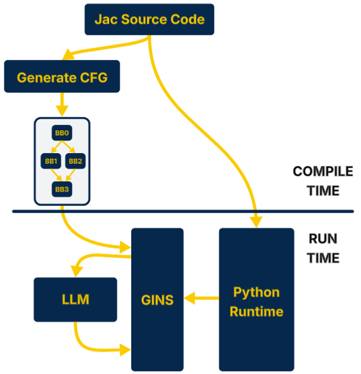
\includegraphics[width=0.5\linewidth]{images/Picture1.png}
    \caption{Design of original implementation of GinS. Note analysis occuring both at compile time and runtime.}
    \label{fig:enter-label}
\end{figure}

This project is implemented upon a previous CSE 583 semeseter project entitled Ghost in the Shell: A Framework to Prompt LLMs at Runtime with Dynamic Information.
In this project, the group developed a Ghost in the Shell (GinS) thread in the Jac programming language.
The general design of this project can be seen in Figure X.
Before the target program began (i.e. during compile time), GinS would construct a CFG for the program.
The GinS thread would then run alongside a Python runtime and gather profiling data on it.
This data would then be used to prompt an LLM in real time to request improvement recommendations as well as hot path analysis and error detection.
Our goal in the project discussed in this paper was to provide more detailed analysis of the GinS performance as well as expand its capabilities both in profiling information collected as well as how that information is used.

\section{Expansions on GinS}

\subsection{Additional Runtime Metrics}
\subsubsection{Tracing Granularity}
The original GinS implementation only used one type of tracing granularity. This involved a callback function that was called each time an instruction was executed in the Python runtime. This enabled very fine granularity, but resulted in significant overhead. An additional level of tracing granularity was tried in this iteration of the project. This involved using a timer as a signal to call a profiling function. This lead to lower granularity but also significantly lower overhead. These tracing granularities were relevant to which profiling metrics were able to be recorded as discussed in later sections.

\subsection{Updated Prompt Formatting}

\subsection{Smart Assertions}

\section{Evaluation}

\subsection{Prompt Formatting Performance}

\subsection{Smart Assertions Performance}

\subsection{GinS Overhead}

\section{Conclusion and Future Work}

%%
%% The acknowledgments section is defined using the "acks" environment
%% (and NOT an unnumbered section). This ensures the proper
%% identification of the section in the article metadata, and the
%% consistent spelling of the heading.
\begin{acks}
Acknowledgements go here. Delete enclosing begin/end markers if there are no acknowledgements.
\end{acks}

%%
%% The next two lines define the bibliography style to be used, and
%% the bibliography file.
\bibliographystyle{ACM-Reference-Format}
\bibliography{references.bib}

%%
\end{document}
\endinput
%%
%% End of file `main.tex'.
